% Seminar 1: Data, returns and indicators
% Statistics of Financial Markets -- Bachelor's programme, Bucharest University of Economic Studies
% GENERATED by latex/build_seminar1.py -- edit the generator, not this file.
% Student version by default; the instructor version is the *_solutions.tex wrapper.
\makeatletter\@ifundefined{ifsolutions}{\expandafter\newif\csname ifsolutions\endcsname}{}\makeatother

\newcommand{\coursename}{Statistics of Financial Markets}
% Preambul comun SFM -- Statistica piețelor financiare / Statistics of Financial Markets (Beamer, 16:9)
% Același design ca MFM. Înainte de % Preambul comun SFM -- Statistica piețelor financiare / Statistics of Financial Markets (Beamer, 16:9)
% Același design ca MFM. Înainte de % Preambul comun SFM -- Statistica piețelor financiare / Statistics of Financial Markets (Beamer, 16:9)
% Același design ca MFM. Înainte de \input{../../latex/preamble} se definește
%   \newcommand{\coursename}{Statistics of Financial Markets}      (EN)
%   \newcommand{\coursename}{Statistica piețelor financiare}       (RO)  și  \def\sfmlang{ro}
% Fișierele .tex se află în EN/Courses, EN/Seminars, RO/Cursuri, RO/Seminarii (două niveluri sub rădăcină).
% Deck-urile sînt generate de latex/build_chapterN.py / build_seminarN.py (vezi latex/sfm_build.py).

\documentclass[9pt, aspectratio=169, t]{beamer}
\providecommand{\coursename}{Statistics of Financial Markets}

% Ensure content fits on slides
\setbeamersize{text margin left=8mm, text margin right=8mm}

%=============================================================================
% THEME AND STYLE CONFIGURATION
%=============================================================================
\usetheme{default}
% Using default theme for clean header/footer control

% Color Palette (matching Redispatch PDF)
\definecolor{MainBlue}{RGB}{26, 58, 110}
\definecolor{AccentBlue}{RGB}{26, 58, 110}
\definecolor{IDAred}{RGB}{205, 0, 0}
\definecolor{DarkGray}{RGB}{51, 51, 51}
\definecolor{MediumGray}{RGB}{128, 128, 128}
\definecolor{LightGray}{RGB}{248, 248, 248}
\definecolor{VeryLightGray}{RGB}{235, 235, 235}
\definecolor{KeynoteGray}{RGB}{218, 218, 218}
\definecolor{SectionGray}{RGB}{120, 120, 120}
\definecolor{FooterGray}{RGB}{100, 100, 100}
\definecolor{Crimson}{RGB}{220, 53, 69}
\definecolor{Forest}{RGB}{46, 125, 50}
\definecolor{Amber}{RGB}{181, 133, 63}
\definecolor{Orange}{RGB}{230, 126, 34}
\definecolor{Purple}{RGB}{142, 68, 173}

% Gradient background (exact Keynote 315° gradient: white to RGB 218,218,218)
\setbeamertemplate{background}{%
    \begin{tikzpicture}[remember picture, overlay]
        \shade[shading=axis, shading angle=315,
        top color=white, bottom color=KeynoteGray]
        (current page.south west) rectangle (current page.north east);
    \end{tikzpicture}%
}
% Fallback solid color for compatibility
\setbeamercolor{background canvas}{bg=}

\setbeamercolor{palette primary}{bg=MainBlue, fg=white}
\setbeamercolor{palette secondary}{bg=MainBlue!85, fg=white}
\setbeamercolor{palette tertiary}{bg=MainBlue!70, fg=white}
\setbeamercolor{structure}{fg=MainBlue}
\setbeamercolor{title}{fg=IDAred}
\setbeamercolor{frametitle}{fg=IDAred, bg=}
\setbeamercolor{block title}{bg=MainBlue, fg=white}
\setbeamercolor{block body}{bg=VeryLightGray, fg=DarkGray}
\setbeamercolor{block title alerted}{bg=Crimson, fg=white}
\setbeamercolor{block body alerted}{bg=Crimson!8, fg=DarkGray}
\setbeamercolor{block title example}{bg=Forest, fg=white}
\setbeamercolor{block body example}{bg=Forest!8, fg=DarkGray}
\setbeamercolor{item}{fg=MainBlue}

% Footer colors (override Madrid theme blue)
\setbeamercolor{author in head/foot}{fg=FooterGray, bg=}
\setbeamercolor{title in head/foot}{fg=FooterGray, bg=}
\setbeamercolor{date in head/foot}{fg=FooterGray, bg=}
\setbeamercolor{section in head/foot}{fg=FooterGray, bg=}
\setbeamercolor{subsection in head/foot}{fg=FooterGray, bg=}

% Bullet styles (apply everywhere including blocks)
\setbeamertemplate{itemize item}{\color{MainBlue}$\boxdot$}
\setbeamertemplate{itemize subitem}{\color{MainBlue}$\blacktriangleright$}
\setbeamertemplate{itemize subsubitem}{\color{MainBlue}\tiny$\bullet$}
\setbeamertemplate{itemize/enumerate body begin}{\normalsize}
\setbeamertemplate{itemize/enumerate subbody begin}{\normalsize}

% Item spacing - compact style
\setlength{\leftmargini}{10pt}       % Level 1: minimal indent
\setlength{\leftmarginii}{10pt}      % Level 2: minimal additional indent
% Compact list spacing (zero extra space before/after lists in blocks)
\makeatletter
\def\@listi{\leftmargin\leftmargini \topsep 0pt \parsep 0pt \itemsep 0pt}
\def\@listii{\leftmargin\leftmarginii \topsep 0pt \parsep 0pt \itemsep 0pt}
\makeatother

\setbeamertemplate{navigation symbols}{}

%=============================================================================
% CUSTOM HEADLINE
%=============================================================================
\setbeamertemplate{headline}{%
    \vskip10pt%
    \hbox to \paperwidth{%
        \hskip0.5cm%
        {\small\color{FooterGray}\renewcommand{\hyperlink}[2]{##2}\insertsectionhead}%
        \hfill%
        \textcolor{FooterGray}{\small\insertframenumber}%
        \hskip0.5cm%
    }%
    \vskip4pt%
    {\color{FooterGray}\hrule height 0.4pt}%
}

%=============================================================================
% CUSTOM FOOTER
%=============================================================================
\usepackage{fontawesome5}

\setbeamertemplate{footline}{%
    {\color{FooterGray}\hrule height 0.4pt}%
    \vskip4pt%
    \hbox to \paperwidth{%
        \hskip0.5cm%
        \textcolor{FooterGray}{\small\coursename}%
        \hfill%
        \raisebox{-0.1em}{%
            \begin{tikzpicture}[x=0.08em, y=0.08em, line width=0.4pt]
                \draw[FooterGray] (0,3) -- (1,4) -- (2,3.5) -- (3,5) -- (4,4) -- (5,6) -- (6,5.5) -- (7,4) -- (8,5) -- (9,7) -- (10,6) -- (11,5) -- (12,6.5) -- (13,8) -- (14,7) -- (15,6) -- (16,7.5) -- (17,9) -- (18,8) -- (19,7) -- (20,8.5) -- (21,10) -- (22,9) -- (23,8) -- (24,9.5);
            \end{tikzpicture}%
        }%
        \hskip0.5cm%
    }%
    \vskip6pt%
}

%=============================================================================
% PACKAGES
%=============================================================================
\usepackage[utf8]{inputenc}
\DeclareUnicodeCharacter{03B1}{\ensuremath{\alpha}}
\usepackage[T1]{fontenc}
\usepackage{amsmath, amssymb, amsthm}
\usepackage{mathtools}
\usepackage{bm}
\usepackage{tikz}
\usetikzlibrary{arrows.meta, positioning, shapes, calc, decorations.pathreplacing, shadings}
\usepackage{booktabs}
\usepackage{multirow}
\usepackage{array}
\usepackage{graphicx}
\usepackage{hyperref}
\usepackage{colortbl}
\usepackage{listings}
\lstset{language=Python, basicstyle=\ttfamily\scriptsize, keywordstyle=\color{MainBlue}\bfseries,
  commentstyle=\color{Forest}, stringstyle=\color{Crimson}, breaklines=true,
  frame=none, backgroundcolor=\color{VeryLightGray}, xleftmargin=2mm}
\hypersetup{colorlinks=true, linkcolor=MainBlue, urlcolor=MainBlue}
\graphicspath{{../../logos/}{../../charts/}{../../photos/}}
\usepackage{xcolor}
\hfuzz=2pt  % Suppress tiny overfull warnings (<2pt)
\vfuzz=2pt  % Suppress tiny vertical overfull warnings (<2pt)

%=============================================================================
% QUANTLET COMMANDS
%   \quantlet{<displayed name>}{<url>}       (generic, compatible with the older SFM decks)
%   \sfmquantlet{Ch_05}{SFM_ch5_garch}       -> https://github.com/danpele/SFM/tree/main/Quantlets/Ch_05/SFM_ch5_garch
%   \qlurl{<folder>} is defined per chapter by the generator (Quantlets/Ch_NN/<folder>)
%=============================================================================
\newcommand{\sfmrepo}{https://github.com/danpele/SFM}
\newcommand{\sfmqlbase}{https://github.com/danpele/SFM/tree/main/Quantlets}
\newcommand{\quantlet}[2]{%
    \hfill\href{#2}{%
        \raisebox{-0.15em}{
\includegraphics[height=0.7em]{ql_logo.png}}%
        \textcolor{MainBlue}{\tiny\ #1}%
    }%
}
\newcommand{\sfmquantlet}[2]{\quantlet{\detokenize{#2}}{\sfmqlbase/#1/#2}}

%=============================================================================
% NOTEBOOKS (Google Colab)
%   \colaburl{notebooks/EN/chapter5_seminar_notebook.ipynb} -> the Colab link of a file in the SFM repo
%   \nb: the chapter notebook (each seminar deck redefines it with \renewcommand)
%=============================================================================
\newcommand{\colaburl}[1]{https://colab.research.google.com/github/danpele/SFM/blob/main/#1}
\newcommand{\nb}{https://colab.research.google.com/github/danpele/SFM/tree/main/notebooks/EN}
\newcommand{\nbname}{notebooks/EN}

%=============================================================================
% SLIDE HELPERS (used by the generators; the same as in MFM)
%=============================================================================
% local font size for list bodies (the preamble forces \normalsize)
\newcommand{\itemsize}[1]{\setbeamertemplate{itemize/enumerate body begin}{#1}\setbeamertemplate{itemize/enumerate subbody begin}{#1}}
\newcommand{\intitle}[1]{{\hypersetup{urlcolor=white}#1}}   % white links inside coloured title bars
\newcommand{\imgcap}[1]{{\scriptsize #1}\\[0.5mm]}          % caption under a photo
\newcommand{\imgcredit}[2]{{\tiny\color{FooterGray}\href{#1}{#2}}}   % image credit: source URL, author/licence
\newcommand{\aiprompt}[1]{{\ttfamily\color{MainBlue}#1}}     % a prompt to an AI assistant

%=============================================================================
% SEMINARS: student version by default; the instructor wrapper *_solutions.tex sets \solutionstrue
%=============================================================================
\makeatletter\@ifundefined{ifsolutions}{\expandafter\newif\csname ifsolutions\endcsname}{}\makeatother
\newcommand{\solonly}[1]{\ifsolutions #1\fi}
\newcommand{\propsub}{\ifsolutions\else\framesubtitle{\ifdefined\sfmlang Rezolvarea se discută la seminar\else Solution discussed in class\fi}\fi}

%=============================================================================
% APPENDIX AND CHAPTER LINKS (latex/appendix_links.py writes the calls; it also re-declares these
% macros before \begin{document}, so the decks compile with or without this preamble block)
%=============================================================================
\providecommand{\sfmapplink}[3]{\hypertarget{#2}{}\hyperlink{#1}{\beamergotobutton{#3}}}
\providecommand{\sfmappback}[2]{\begin{tikzpicture}[remember picture,overlay]\node[anchor=south east] at ([xshift=-3mm,yshift=7mm]current page.south east){\hyperlink{#1}{\beamerreturnbutton{#2}}};\end{tikzpicture}}
\providecommand{\sfmchlink}[2]{\href{#1}{#2}}
\providecommand{\sfmchlinkt}[2]{\href{#1}{\usebeamercolor[fg]{frametitle}#2}}

%=============================================================================
% QUANTINAR COMMAND: link către un curs Quantinar (subiecte avansate)
%=============================================================================
\newcommand{\quantinar}[2]{%
    \href{#2}{%
        \raisebox{-0.15em}{
\includegraphics[height=0.8em]{qr_logo.png}}%
        \textcolor{MainBlue}{\scriptsize\ #1}%
    }%
}

%=============================================================================
% CUSTOM TITLE PAGE
%=============================================================================
\defbeamertemplate*{title page}{hybrid}[1][]
{
    \vspace{0.2cm}
    % Logos row - top header (with clickable links)
    \begin{center}
        \href{https://www.ase.ro}{
\includegraphics[height=1.0cm]{ase_logo.png}}\hspace{0.3cm}%
        \href{https://theida.net}{
\includegraphics[height=1.0cm]{ida_logo.png}}\hspace{0.3cm}%
        \href{https://blockchain-research-center.com}{
\includegraphics[height=1.0cm]{brc_logo.png}}\hspace{0.3cm}%
        \href{https://www.ai4efin.ase.ro}{
\includegraphics[height=1.0cm]{ai4efin_logo.png}}\hspace{0.3cm}%
        \href{https://ipe.ro/new}{
\includegraphics[height=1.0cm]{acad_logo.png}}\hspace{0.3cm}%
        \href{https://www.digital-finance-msca.com}{
\includegraphics[height=1.0cm]{msca_logo.png}}%
    \end{center}

    \vspace{0.6cm}

    % Main title with Q logos on sides (with clickable links)
    \begin{center}
        \begin{minipage}{0.1\textwidth}
            \centering
            \href{https://quantlet.com}{
\includegraphics[height=1.1cm]{ql_logo.png}}
        \end{minipage}%
        \begin{minipage}{0.78\textwidth}
            \centering
            {\LARGE\bfseries\usebeamercolor[fg]{title}\inserttitle}

            \vspace{0.3cm}

            {\usebeamerfont{subtitle}\usebeamercolor[fg]{title}\insertsubtitle}
        \end{minipage}%
        \begin{minipage}{0.1\textwidth}
            \centering
            \href{https://quantinar.com}{
\includegraphics[height=1.1cm]{qr_logo.png}}
        \end{minipage}
    \end{center}

    \vspace{0.6cm}

    % Authors (left aligned)
    \hspace{0.5cm}{\usebeamerfont{author}\insertauthor}

    \vspace{0.3cm}

    % Institute/Affiliations (left aligned)
    \hspace{0.5cm}\begin{minipage}[t]{0.9\textwidth}
        \raggedright\small\insertinstitute
    \end{minipage}
}

%=============================================================================
% THEOREM ENVIRONMENTS
%=============================================================================
\theoremstyle{definition}
\setbeamertemplate{theorems}[numbered]
\ifdefined\sfmlang
\newtheorem{defn}{Definiție}
\newtheorem{thm}{Teoremă}
\newtheorem{prop}{Propoziție}
\newtheorem{rmk}{Observație}
\else
\newtheorem{defn}{Definition}
\newtheorem{thm}{Theorem}
\newtheorem{prop}{Proposition}
\newtheorem{rmk}{Remark}
\fi

%=============================================================================
% CENTRED MINIPAGE (no extra vertical space)
%=============================================================================
\newenvironment{cminipage}[1]{%
    \par\noindent\hfill\begin{minipage}{#1}\ignorespaces
}{%
    \end{minipage}\hfill\null\par
}

%=============================================================================
% CUSTOM COMMANDS
%=============================================================================
\newcommand{\E}{\mathbb{E}}
\newcommand{\Var}{\text{Var}}
\newcommand{\Cov}{\text{Cov}}
\newcommand{\Corr}{\text{Corr}}
\newcommand{\R}{\mathbb{R}}
\newcommand{\N}{\mathbb{N}}
\newcommand{\Z}{\mathbb{Z}}
\newcommand{\B}{\mathbf{B}}
\newcommand{\imark}{\textcolor{MainBlue}{\textbullet}}
\newcommand{\RMSE}{\text{RMSE}}
\newcommand{\MAE}{\text{MAE}}
\newcommand{\MAPE}{\text{MAPE}}

 se definește
%   \newcommand{\coursename}{Statistics of Financial Markets}      (EN)
%   \newcommand{\coursename}{Statistica piețelor financiare}       (RO)  și  \def\sfmlang{ro}
% Fișierele .tex se află în EN/Courses, EN/Seminars, RO/Cursuri, RO/Seminarii (două niveluri sub rădăcină).
% Deck-urile sînt generate de latex/build_chapterN.py / build_seminarN.py (vezi latex/sfm_build.py).

\documentclass[9pt, aspectratio=169, t]{beamer}
\providecommand{\coursename}{Statistics of Financial Markets}

% Ensure content fits on slides
\setbeamersize{text margin left=8mm, text margin right=8mm}

%=============================================================================
% THEME AND STYLE CONFIGURATION
%=============================================================================
\usetheme{default}
% Using default theme for clean header/footer control

% Color Palette (matching Redispatch PDF)
\definecolor{MainBlue}{RGB}{26, 58, 110}
\definecolor{AccentBlue}{RGB}{26, 58, 110}
\definecolor{IDAred}{RGB}{205, 0, 0}
\definecolor{DarkGray}{RGB}{51, 51, 51}
\definecolor{MediumGray}{RGB}{128, 128, 128}
\definecolor{LightGray}{RGB}{248, 248, 248}
\definecolor{VeryLightGray}{RGB}{235, 235, 235}
\definecolor{KeynoteGray}{RGB}{218, 218, 218}
\definecolor{SectionGray}{RGB}{120, 120, 120}
\definecolor{FooterGray}{RGB}{100, 100, 100}
\definecolor{Crimson}{RGB}{220, 53, 69}
\definecolor{Forest}{RGB}{46, 125, 50}
\definecolor{Amber}{RGB}{181, 133, 63}
\definecolor{Orange}{RGB}{230, 126, 34}
\definecolor{Purple}{RGB}{142, 68, 173}

% Gradient background (exact Keynote 315° gradient: white to RGB 218,218,218)
\setbeamertemplate{background}{%
    \begin{tikzpicture}[remember picture, overlay]
        \shade[shading=axis, shading angle=315,
        top color=white, bottom color=KeynoteGray]
        (current page.south west) rectangle (current page.north east);
    \end{tikzpicture}%
}
% Fallback solid color for compatibility
\setbeamercolor{background canvas}{bg=}

\setbeamercolor{palette primary}{bg=MainBlue, fg=white}
\setbeamercolor{palette secondary}{bg=MainBlue!85, fg=white}
\setbeamercolor{palette tertiary}{bg=MainBlue!70, fg=white}
\setbeamercolor{structure}{fg=MainBlue}
\setbeamercolor{title}{fg=IDAred}
\setbeamercolor{frametitle}{fg=IDAred, bg=}
\setbeamercolor{block title}{bg=MainBlue, fg=white}
\setbeamercolor{block body}{bg=VeryLightGray, fg=DarkGray}
\setbeamercolor{block title alerted}{bg=Crimson, fg=white}
\setbeamercolor{block body alerted}{bg=Crimson!8, fg=DarkGray}
\setbeamercolor{block title example}{bg=Forest, fg=white}
\setbeamercolor{block body example}{bg=Forest!8, fg=DarkGray}
\setbeamercolor{item}{fg=MainBlue}

% Footer colors (override Madrid theme blue)
\setbeamercolor{author in head/foot}{fg=FooterGray, bg=}
\setbeamercolor{title in head/foot}{fg=FooterGray, bg=}
\setbeamercolor{date in head/foot}{fg=FooterGray, bg=}
\setbeamercolor{section in head/foot}{fg=FooterGray, bg=}
\setbeamercolor{subsection in head/foot}{fg=FooterGray, bg=}

% Bullet styles (apply everywhere including blocks)
\setbeamertemplate{itemize item}{\color{MainBlue}$\boxdot$}
\setbeamertemplate{itemize subitem}{\color{MainBlue}$\blacktriangleright$}
\setbeamertemplate{itemize subsubitem}{\color{MainBlue}\tiny$\bullet$}
\setbeamertemplate{itemize/enumerate body begin}{\normalsize}
\setbeamertemplate{itemize/enumerate subbody begin}{\normalsize}

% Item spacing - compact style
\setlength{\leftmargini}{10pt}       % Level 1: minimal indent
\setlength{\leftmarginii}{10pt}      % Level 2: minimal additional indent
% Compact list spacing (zero extra space before/after lists in blocks)
\makeatletter
\def\@listi{\leftmargin\leftmargini \topsep 0pt \parsep 0pt \itemsep 0pt}
\def\@listii{\leftmargin\leftmarginii \topsep 0pt \parsep 0pt \itemsep 0pt}
\makeatother

\setbeamertemplate{navigation symbols}{}

%=============================================================================
% CUSTOM HEADLINE
%=============================================================================
\setbeamertemplate{headline}{%
    \vskip10pt%
    \hbox to \paperwidth{%
        \hskip0.5cm%
        {\small\color{FooterGray}\renewcommand{\hyperlink}[2]{##2}\insertsectionhead}%
        \hfill%
        \textcolor{FooterGray}{\small\insertframenumber}%
        \hskip0.5cm%
    }%
    \vskip4pt%
    {\color{FooterGray}\hrule height 0.4pt}%
}

%=============================================================================
% CUSTOM FOOTER
%=============================================================================
\usepackage{fontawesome5}

\setbeamertemplate{footline}{%
    {\color{FooterGray}\hrule height 0.4pt}%
    \vskip4pt%
    \hbox to \paperwidth{%
        \hskip0.5cm%
        \textcolor{FooterGray}{\small\coursename}%
        \hfill%
        \raisebox{-0.1em}{%
            \begin{tikzpicture}[x=0.08em, y=0.08em, line width=0.4pt]
                \draw[FooterGray] (0,3) -- (1,4) -- (2,3.5) -- (3,5) -- (4,4) -- (5,6) -- (6,5.5) -- (7,4) -- (8,5) -- (9,7) -- (10,6) -- (11,5) -- (12,6.5) -- (13,8) -- (14,7) -- (15,6) -- (16,7.5) -- (17,9) -- (18,8) -- (19,7) -- (20,8.5) -- (21,10) -- (22,9) -- (23,8) -- (24,9.5);
            \end{tikzpicture}%
        }%
        \hskip0.5cm%
    }%
    \vskip6pt%
}

%=============================================================================
% PACKAGES
%=============================================================================
\usepackage[utf8]{inputenc}
\DeclareUnicodeCharacter{03B1}{\ensuremath{\alpha}}
\usepackage[T1]{fontenc}
\usepackage{amsmath, amssymb, amsthm}
\usepackage{mathtools}
\usepackage{bm}
\usepackage{tikz}
\usetikzlibrary{arrows.meta, positioning, shapes, calc, decorations.pathreplacing, shadings}
\usepackage{booktabs}
\usepackage{multirow}
\usepackage{array}
\usepackage{graphicx}
\usepackage{hyperref}
\usepackage{colortbl}
\usepackage{listings}
\lstset{language=Python, basicstyle=\ttfamily\scriptsize, keywordstyle=\color{MainBlue}\bfseries,
  commentstyle=\color{Forest}, stringstyle=\color{Crimson}, breaklines=true,
  frame=none, backgroundcolor=\color{VeryLightGray}, xleftmargin=2mm}
\hypersetup{colorlinks=true, linkcolor=MainBlue, urlcolor=MainBlue}
\graphicspath{{../../logos/}{../../charts/}{../../photos/}}
\usepackage{xcolor}
\hfuzz=2pt  % Suppress tiny overfull warnings (<2pt)
\vfuzz=2pt  % Suppress tiny vertical overfull warnings (<2pt)

%=============================================================================
% QUANTLET COMMANDS
%   \quantlet{<displayed name>}{<url>}       (generic, compatible with the older SFM decks)
%   \sfmquantlet{Ch_05}{SFM_ch5_garch}       -> https://github.com/danpele/SFM/tree/main/Quantlets/Ch_05/SFM_ch5_garch
%   \qlurl{<folder>} is defined per chapter by the generator (Quantlets/Ch_NN/<folder>)
%=============================================================================
\newcommand{\sfmrepo}{https://github.com/danpele/SFM}
\newcommand{\sfmqlbase}{https://github.com/danpele/SFM/tree/main/Quantlets}
\newcommand{\quantlet}[2]{%
    \hfill\href{#2}{%
        \raisebox{-0.15em}{
\includegraphics[height=0.7em]{ql_logo.png}}%
        \textcolor{MainBlue}{\tiny\ #1}%
    }%
}
\newcommand{\sfmquantlet}[2]{\quantlet{\detokenize{#2}}{\sfmqlbase/#1/#2}}

%=============================================================================
% NOTEBOOKS (Google Colab)
%   \colaburl{notebooks/EN/chapter5_seminar_notebook.ipynb} -> the Colab link of a file in the SFM repo
%   \nb: the chapter notebook (each seminar deck redefines it with \renewcommand)
%=============================================================================
\newcommand{\colaburl}[1]{https://colab.research.google.com/github/danpele/SFM/blob/main/#1}
\newcommand{\nb}{https://colab.research.google.com/github/danpele/SFM/tree/main/notebooks/EN}
\newcommand{\nbname}{notebooks/EN}

%=============================================================================
% SLIDE HELPERS (used by the generators; the same as in MFM)
%=============================================================================
% local font size for list bodies (the preamble forces \normalsize)
\newcommand{\itemsize}[1]{\setbeamertemplate{itemize/enumerate body begin}{#1}\setbeamertemplate{itemize/enumerate subbody begin}{#1}}
\newcommand{\intitle}[1]{{\hypersetup{urlcolor=white}#1}}   % white links inside coloured title bars
\newcommand{\imgcap}[1]{{\scriptsize #1}\\[0.5mm]}          % caption under a photo
\newcommand{\imgcredit}[2]{{\tiny\color{FooterGray}\href{#1}{#2}}}   % image credit: source URL, author/licence
\newcommand{\aiprompt}[1]{{\ttfamily\color{MainBlue}#1}}     % a prompt to an AI assistant

%=============================================================================
% SEMINARS: student version by default; the instructor wrapper *_solutions.tex sets \solutionstrue
%=============================================================================
\makeatletter\@ifundefined{ifsolutions}{\expandafter\newif\csname ifsolutions\endcsname}{}\makeatother
\newcommand{\solonly}[1]{\ifsolutions #1\fi}
\newcommand{\propsub}{\ifsolutions\else\framesubtitle{\ifdefined\sfmlang Rezolvarea se discută la seminar\else Solution discussed in class\fi}\fi}

%=============================================================================
% APPENDIX AND CHAPTER LINKS (latex/appendix_links.py writes the calls; it also re-declares these
% macros before \begin{document}, so the decks compile with or without this preamble block)
%=============================================================================
\providecommand{\sfmapplink}[3]{\hypertarget{#2}{}\hyperlink{#1}{\beamergotobutton{#3}}}
\providecommand{\sfmappback}[2]{\begin{tikzpicture}[remember picture,overlay]\node[anchor=south east] at ([xshift=-3mm,yshift=7mm]current page.south east){\hyperlink{#1}{\beamerreturnbutton{#2}}};\end{tikzpicture}}
\providecommand{\sfmchlink}[2]{\href{#1}{#2}}
\providecommand{\sfmchlinkt}[2]{\href{#1}{\usebeamercolor[fg]{frametitle}#2}}

%=============================================================================
% QUANTINAR COMMAND: link către un curs Quantinar (subiecte avansate)
%=============================================================================
\newcommand{\quantinar}[2]{%
    \href{#2}{%
        \raisebox{-0.15em}{
\includegraphics[height=0.8em]{qr_logo.png}}%
        \textcolor{MainBlue}{\scriptsize\ #1}%
    }%
}

%=============================================================================
% CUSTOM TITLE PAGE
%=============================================================================
\defbeamertemplate*{title page}{hybrid}[1][]
{
    \vspace{0.2cm}
    % Logos row - top header (with clickable links)
    \begin{center}
        \href{https://www.ase.ro}{
\includegraphics[height=1.0cm]{ase_logo.png}}\hspace{0.3cm}%
        \href{https://theida.net}{
\includegraphics[height=1.0cm]{ida_logo.png}}\hspace{0.3cm}%
        \href{https://blockchain-research-center.com}{
\includegraphics[height=1.0cm]{brc_logo.png}}\hspace{0.3cm}%
        \href{https://www.ai4efin.ase.ro}{
\includegraphics[height=1.0cm]{ai4efin_logo.png}}\hspace{0.3cm}%
        \href{https://ipe.ro/new}{
\includegraphics[height=1.0cm]{acad_logo.png}}\hspace{0.3cm}%
        \href{https://www.digital-finance-msca.com}{
\includegraphics[height=1.0cm]{msca_logo.png}}%
    \end{center}

    \vspace{0.6cm}

    % Main title with Q logos on sides (with clickable links)
    \begin{center}
        \begin{minipage}{0.1\textwidth}
            \centering
            \href{https://quantlet.com}{
\includegraphics[height=1.1cm]{ql_logo.png}}
        \end{minipage}%
        \begin{minipage}{0.78\textwidth}
            \centering
            {\LARGE\bfseries\usebeamercolor[fg]{title}\inserttitle}

            \vspace{0.3cm}

            {\usebeamerfont{subtitle}\usebeamercolor[fg]{title}\insertsubtitle}
        \end{minipage}%
        \begin{minipage}{0.1\textwidth}
            \centering
            \href{https://quantinar.com}{
\includegraphics[height=1.1cm]{qr_logo.png}}
        \end{minipage}
    \end{center}

    \vspace{0.6cm}

    % Authors (left aligned)
    \hspace{0.5cm}{\usebeamerfont{author}\insertauthor}

    \vspace{0.3cm}

    % Institute/Affiliations (left aligned)
    \hspace{0.5cm}\begin{minipage}[t]{0.9\textwidth}
        \raggedright\small\insertinstitute
    \end{minipage}
}

%=============================================================================
% THEOREM ENVIRONMENTS
%=============================================================================
\theoremstyle{definition}
\setbeamertemplate{theorems}[numbered]
\ifdefined\sfmlang
\newtheorem{defn}{Definiție}
\newtheorem{thm}{Teoremă}
\newtheorem{prop}{Propoziție}
\newtheorem{rmk}{Observație}
\else
\newtheorem{defn}{Definition}
\newtheorem{thm}{Theorem}
\newtheorem{prop}{Proposition}
\newtheorem{rmk}{Remark}
\fi

%=============================================================================
% CENTRED MINIPAGE (no extra vertical space)
%=============================================================================
\newenvironment{cminipage}[1]{%
    \par\noindent\hfill\begin{minipage}{#1}\ignorespaces
}{%
    \end{minipage}\hfill\null\par
}

%=============================================================================
% CUSTOM COMMANDS
%=============================================================================
\newcommand{\E}{\mathbb{E}}
\newcommand{\Var}{\text{Var}}
\newcommand{\Cov}{\text{Cov}}
\newcommand{\Corr}{\text{Corr}}
\newcommand{\R}{\mathbb{R}}
\newcommand{\N}{\mathbb{N}}
\newcommand{\Z}{\mathbb{Z}}
\newcommand{\B}{\mathbf{B}}
\newcommand{\imark}{\textcolor{MainBlue}{\textbullet}}
\newcommand{\RMSE}{\text{RMSE}}
\newcommand{\MAE}{\text{MAE}}
\newcommand{\MAPE}{\text{MAPE}}

 se definește
%   \newcommand{\coursename}{Statistics of Financial Markets}      (EN)
%   \newcommand{\coursename}{Statistica piețelor financiare}       (RO)  și  \def\sfmlang{ro}
% Fișierele .tex se află în EN/Courses, EN/Seminars, RO/Cursuri, RO/Seminarii (două niveluri sub rădăcină).
% Deck-urile sînt generate de latex/build_chapterN.py / build_seminarN.py (vezi latex/sfm_build.py).

\documentclass[9pt, aspectratio=169, t]{beamer}
\providecommand{\coursename}{Statistics of Financial Markets}

% Ensure content fits on slides
\setbeamersize{text margin left=8mm, text margin right=8mm}

%=============================================================================
% THEME AND STYLE CONFIGURATION
%=============================================================================
\usetheme{default}
% Using default theme for clean header/footer control

% Color Palette (matching Redispatch PDF)
\definecolor{MainBlue}{RGB}{26, 58, 110}
\definecolor{AccentBlue}{RGB}{26, 58, 110}
\definecolor{IDAred}{RGB}{205, 0, 0}
\definecolor{DarkGray}{RGB}{51, 51, 51}
\definecolor{MediumGray}{RGB}{128, 128, 128}
\definecolor{LightGray}{RGB}{248, 248, 248}
\definecolor{VeryLightGray}{RGB}{235, 235, 235}
\definecolor{KeynoteGray}{RGB}{218, 218, 218}
\definecolor{SectionGray}{RGB}{120, 120, 120}
\definecolor{FooterGray}{RGB}{100, 100, 100}
\definecolor{Crimson}{RGB}{220, 53, 69}
\definecolor{Forest}{RGB}{46, 125, 50}
\definecolor{Amber}{RGB}{181, 133, 63}
\definecolor{Orange}{RGB}{230, 126, 34}
\definecolor{Purple}{RGB}{142, 68, 173}

% Gradient background (exact Keynote 315° gradient: white to RGB 218,218,218)
\setbeamertemplate{background}{%
    \begin{tikzpicture}[remember picture, overlay]
        \shade[shading=axis, shading angle=315,
        top color=white, bottom color=KeynoteGray]
        (current page.south west) rectangle (current page.north east);
    \end{tikzpicture}%
}
% Fallback solid color for compatibility
\setbeamercolor{background canvas}{bg=}

\setbeamercolor{palette primary}{bg=MainBlue, fg=white}
\setbeamercolor{palette secondary}{bg=MainBlue!85, fg=white}
\setbeamercolor{palette tertiary}{bg=MainBlue!70, fg=white}
\setbeamercolor{structure}{fg=MainBlue}
\setbeamercolor{title}{fg=IDAred}
\setbeamercolor{frametitle}{fg=IDAred, bg=}
\setbeamercolor{block title}{bg=MainBlue, fg=white}
\setbeamercolor{block body}{bg=VeryLightGray, fg=DarkGray}
\setbeamercolor{block title alerted}{bg=Crimson, fg=white}
\setbeamercolor{block body alerted}{bg=Crimson!8, fg=DarkGray}
\setbeamercolor{block title example}{bg=Forest, fg=white}
\setbeamercolor{block body example}{bg=Forest!8, fg=DarkGray}
\setbeamercolor{item}{fg=MainBlue}

% Footer colors (override Madrid theme blue)
\setbeamercolor{author in head/foot}{fg=FooterGray, bg=}
\setbeamercolor{title in head/foot}{fg=FooterGray, bg=}
\setbeamercolor{date in head/foot}{fg=FooterGray, bg=}
\setbeamercolor{section in head/foot}{fg=FooterGray, bg=}
\setbeamercolor{subsection in head/foot}{fg=FooterGray, bg=}

% Bullet styles (apply everywhere including blocks)
\setbeamertemplate{itemize item}{\color{MainBlue}$\boxdot$}
\setbeamertemplate{itemize subitem}{\color{MainBlue}$\blacktriangleright$}
\setbeamertemplate{itemize subsubitem}{\color{MainBlue}\tiny$\bullet$}
\setbeamertemplate{itemize/enumerate body begin}{\normalsize}
\setbeamertemplate{itemize/enumerate subbody begin}{\normalsize}

% Item spacing - compact style
\setlength{\leftmargini}{10pt}       % Level 1: minimal indent
\setlength{\leftmarginii}{10pt}      % Level 2: minimal additional indent
% Compact list spacing (zero extra space before/after lists in blocks)
\makeatletter
\def\@listi{\leftmargin\leftmargini \topsep 0pt \parsep 0pt \itemsep 0pt}
\def\@listii{\leftmargin\leftmarginii \topsep 0pt \parsep 0pt \itemsep 0pt}
\makeatother

\setbeamertemplate{navigation symbols}{}

%=============================================================================
% CUSTOM HEADLINE
%=============================================================================
\setbeamertemplate{headline}{%
    \vskip10pt%
    \hbox to \paperwidth{%
        \hskip0.5cm%
        {\small\color{FooterGray}\renewcommand{\hyperlink}[2]{##2}\insertsectionhead}%
        \hfill%
        \textcolor{FooterGray}{\small\insertframenumber}%
        \hskip0.5cm%
    }%
    \vskip4pt%
    {\color{FooterGray}\hrule height 0.4pt}%
}

%=============================================================================
% CUSTOM FOOTER
%=============================================================================
\usepackage{fontawesome5}

\setbeamertemplate{footline}{%
    {\color{FooterGray}\hrule height 0.4pt}%
    \vskip4pt%
    \hbox to \paperwidth{%
        \hskip0.5cm%
        \textcolor{FooterGray}{\small\coursename}%
        \hfill%
        \raisebox{-0.1em}{%
            \begin{tikzpicture}[x=0.08em, y=0.08em, line width=0.4pt]
                \draw[FooterGray] (0,3) -- (1,4) -- (2,3.5) -- (3,5) -- (4,4) -- (5,6) -- (6,5.5) -- (7,4) -- (8,5) -- (9,7) -- (10,6) -- (11,5) -- (12,6.5) -- (13,8) -- (14,7) -- (15,6) -- (16,7.5) -- (17,9) -- (18,8) -- (19,7) -- (20,8.5) -- (21,10) -- (22,9) -- (23,8) -- (24,9.5);
            \end{tikzpicture}%
        }%
        \hskip0.5cm%
    }%
    \vskip6pt%
}

%=============================================================================
% PACKAGES
%=============================================================================
\usepackage[utf8]{inputenc}
\DeclareUnicodeCharacter{03B1}{\ensuremath{\alpha}}
\usepackage[T1]{fontenc}
\usepackage{amsmath, amssymb, amsthm}
\usepackage{mathtools}
\usepackage{bm}
\usepackage{tikz}
\usetikzlibrary{arrows.meta, positioning, shapes, calc, decorations.pathreplacing, shadings}
\usepackage{booktabs}
\usepackage{multirow}
\usepackage{array}
\usepackage{graphicx}
\usepackage{hyperref}
\usepackage{colortbl}
\usepackage{listings}
\lstset{language=Python, basicstyle=\ttfamily\scriptsize, keywordstyle=\color{MainBlue}\bfseries,
  commentstyle=\color{Forest}, stringstyle=\color{Crimson}, breaklines=true,
  frame=none, backgroundcolor=\color{VeryLightGray}, xleftmargin=2mm}
\hypersetup{colorlinks=true, linkcolor=MainBlue, urlcolor=MainBlue}
\graphicspath{{../../logos/}{../../charts/}{../../photos/}}
\usepackage{xcolor}
\hfuzz=2pt  % Suppress tiny overfull warnings (<2pt)
\vfuzz=2pt  % Suppress tiny vertical overfull warnings (<2pt)

%=============================================================================
% QUANTLET COMMANDS
%   \quantlet{<displayed name>}{<url>}       (generic, compatible with the older SFM decks)
%   \sfmquantlet{Ch_05}{SFM_ch5_garch}       -> https://github.com/danpele/SFM/tree/main/Quantlets/Ch_05/SFM_ch5_garch
%   \qlurl{<folder>} is defined per chapter by the generator (Quantlets/Ch_NN/<folder>)
%=============================================================================
\newcommand{\sfmrepo}{https://github.com/danpele/SFM}
\newcommand{\sfmqlbase}{https://github.com/danpele/SFM/tree/main/Quantlets}
\newcommand{\quantlet}[2]{%
    \hfill\href{#2}{%
        \raisebox{-0.15em}{
\includegraphics[height=0.7em]{ql_logo.png}}%
        \textcolor{MainBlue}{\tiny\ #1}%
    }%
}
\newcommand{\sfmquantlet}[2]{\quantlet{\detokenize{#2}}{\sfmqlbase/#1/#2}}

%=============================================================================
% NOTEBOOKS (Google Colab)
%   \colaburl{notebooks/EN/chapter5_seminar_notebook.ipynb} -> the Colab link of a file in the SFM repo
%   \nb: the chapter notebook (each seminar deck redefines it with \renewcommand)
%=============================================================================
\newcommand{\colaburl}[1]{https://colab.research.google.com/github/danpele/SFM/blob/main/#1}
\newcommand{\nb}{https://colab.research.google.com/github/danpele/SFM/tree/main/notebooks/EN}
\newcommand{\nbname}{notebooks/EN}

%=============================================================================
% SLIDE HELPERS (used by the generators; the same as in MFM)
%=============================================================================
% local font size for list bodies (the preamble forces \normalsize)
\newcommand{\itemsize}[1]{\setbeamertemplate{itemize/enumerate body begin}{#1}\setbeamertemplate{itemize/enumerate subbody begin}{#1}}
\newcommand{\intitle}[1]{{\hypersetup{urlcolor=white}#1}}   % white links inside coloured title bars
\newcommand{\imgcap}[1]{{\scriptsize #1}\\[0.5mm]}          % caption under a photo
\newcommand{\imgcredit}[2]{{\tiny\color{FooterGray}\href{#1}{#2}}}   % image credit: source URL, author/licence
\newcommand{\aiprompt}[1]{{\ttfamily\color{MainBlue}#1}}     % a prompt to an AI assistant

%=============================================================================
% SEMINARS: student version by default; the instructor wrapper *_solutions.tex sets \solutionstrue
%=============================================================================
\makeatletter\@ifundefined{ifsolutions}{\expandafter\newif\csname ifsolutions\endcsname}{}\makeatother
\newcommand{\solonly}[1]{\ifsolutions #1\fi}
\newcommand{\propsub}{\ifsolutions\else\framesubtitle{\ifdefined\sfmlang Rezolvarea se discută la seminar\else Solution discussed in class\fi}\fi}

%=============================================================================
% APPENDIX AND CHAPTER LINKS (latex/appendix_links.py writes the calls; it also re-declares these
% macros before \begin{document}, so the decks compile with or without this preamble block)
%=============================================================================
\providecommand{\sfmapplink}[3]{\hypertarget{#2}{}\hyperlink{#1}{\beamergotobutton{#3}}}
\providecommand{\sfmappback}[2]{\begin{tikzpicture}[remember picture,overlay]\node[anchor=south east] at ([xshift=-3mm,yshift=7mm]current page.south east){\hyperlink{#1}{\beamerreturnbutton{#2}}};\end{tikzpicture}}
\providecommand{\sfmchlink}[2]{\href{#1}{#2}}
\providecommand{\sfmchlinkt}[2]{\href{#1}{\usebeamercolor[fg]{frametitle}#2}}

%=============================================================================
% QUANTINAR COMMAND: link către un curs Quantinar (subiecte avansate)
%=============================================================================
\newcommand{\quantinar}[2]{%
    \href{#2}{%
        \raisebox{-0.15em}{
\includegraphics[height=0.8em]{qr_logo.png}}%
        \textcolor{MainBlue}{\scriptsize\ #1}%
    }%
}

%=============================================================================
% CUSTOM TITLE PAGE
%=============================================================================
\defbeamertemplate*{title page}{hybrid}[1][]
{
    \vspace{0.2cm}
    % Logos row - top header (with clickable links)
    \begin{center}
        \href{https://www.ase.ro}{
\includegraphics[height=1.0cm]{ase_logo.png}}\hspace{0.3cm}%
        \href{https://theida.net}{
\includegraphics[height=1.0cm]{ida_logo.png}}\hspace{0.3cm}%
        \href{https://blockchain-research-center.com}{
\includegraphics[height=1.0cm]{brc_logo.png}}\hspace{0.3cm}%
        \href{https://www.ai4efin.ase.ro}{
\includegraphics[height=1.0cm]{ai4efin_logo.png}}\hspace{0.3cm}%
        \href{https://ipe.ro/new}{
\includegraphics[height=1.0cm]{acad_logo.png}}\hspace{0.3cm}%
        \href{https://www.digital-finance-msca.com}{
\includegraphics[height=1.0cm]{msca_logo.png}}%
    \end{center}

    \vspace{0.6cm}

    % Main title with Q logos on sides (with clickable links)
    \begin{center}
        \begin{minipage}{0.1\textwidth}
            \centering
            \href{https://quantlet.com}{
\includegraphics[height=1.1cm]{ql_logo.png}}
        \end{minipage}%
        \begin{minipage}{0.78\textwidth}
            \centering
            {\LARGE\bfseries\usebeamercolor[fg]{title}\inserttitle}

            \vspace{0.3cm}

            {\usebeamerfont{subtitle}\usebeamercolor[fg]{title}\insertsubtitle}
        \end{minipage}%
        \begin{minipage}{0.1\textwidth}
            \centering
            \href{https://quantinar.com}{
\includegraphics[height=1.1cm]{qr_logo.png}}
        \end{minipage}
    \end{center}

    \vspace{0.6cm}

    % Authors (left aligned)
    \hspace{0.5cm}{\usebeamerfont{author}\insertauthor}

    \vspace{0.3cm}

    % Institute/Affiliations (left aligned)
    \hspace{0.5cm}\begin{minipage}[t]{0.9\textwidth}
        \raggedright\small\insertinstitute
    \end{minipage}
}

%=============================================================================
% THEOREM ENVIRONMENTS
%=============================================================================
\theoremstyle{definition}
\setbeamertemplate{theorems}[numbered]
\ifdefined\sfmlang
\newtheorem{defn}{Definiție}
\newtheorem{thm}{Teoremă}
\newtheorem{prop}{Propoziție}
\newtheorem{rmk}{Observație}
\else
\newtheorem{defn}{Definition}
\newtheorem{thm}{Theorem}
\newtheorem{prop}{Proposition}
\newtheorem{rmk}{Remark}
\fi

%=============================================================================
% CENTRED MINIPAGE (no extra vertical space)
%=============================================================================
\newenvironment{cminipage}[1]{%
    \par\noindent\hfill\begin{minipage}{#1}\ignorespaces
}{%
    \end{minipage}\hfill\null\par
}

%=============================================================================
% CUSTOM COMMANDS
%=============================================================================
\newcommand{\E}{\mathbb{E}}
\newcommand{\Var}{\text{Var}}
\newcommand{\Cov}{\text{Cov}}
\newcommand{\Corr}{\text{Corr}}
\newcommand{\R}{\mathbb{R}}
\newcommand{\N}{\mathbb{N}}
\newcommand{\Z}{\mathbb{Z}}
\newcommand{\B}{\mathbf{B}}
\newcommand{\imark}{\textcolor{MainBlue}{\textbullet}}
\newcommand{\RMSE}{\text{RMSE}}
\newcommand{\MAE}{\text{MAE}}
\newcommand{\MAPE}{\text{MAPE}}



\newcommand{\qlurl}[1]{https://github.com/danpele/SFM/tree/main/Quantlets/Ch_01/#1}
\renewcommand{\nb}{\colaburl{notebooks/EN/chapter1_seminar_notebook.ipynb}}
\renewcommand{\nbname}{chapter1\_seminar\_notebook.ipynb}
% left column: full width in the student version, narrower next to the solution
\newcommand{\taskw}{\ifsolutions 0.47\textwidth\else 0.96\textwidth\fi}
\newcommand{\solw}{\ifsolutions 0.49\textwidth\else 0pt\fi}

% Clickable citations (DOIs verified via Crossref)

\newcommand{\refFHH}{\href{https://doi.org/10.1007/978-3-030-13751-9}{Franke, Härdle \& Hafner (2019)}}
\newcommand{\refFHHex}{\href{https://doi.org/10.1007/978-3-642-33929-5}{Borak, Härdle \& López-Cabrera (2013)}}
\newcommand{\refTsay}{\href{https://doi.org/10.1002/9780470644560}{Tsay (2010)}}
\newcommand{\refCLM}{\href{https://doi.org/10.1515/9781400830213}{Campbell, Lo \& MacKinlay (1997)}}
\newcommand{\refSharpeA}{\href{https://doi.org/10.1086/294846}{Sharpe (1966)}}
\newcommand{\refSharpeB}{\href{https://doi.org/10.3905/jpm.1994.409501}{Sharpe (1994)}}
\newcommand{\refLo}{\href{https://doi.org/10.2469/faj.v58.n4.2453}{Lo (2002)}}
\newcommand{\refSortino}{\href{https://doi.org/10.3905/jpm.1991.409343}{Sortino \& van der Meer (1991)}}
\newcommand{\refMagdon}{\href{https://doi.org/10.1239/jap/1077134674}{Magdon-Ismail et al.\ (2004)}}
\newcommand{\refCont}{\href{https://doi.org/10.1080/713665670}{Cont (2001)}}
\newcommand{\refBoothFama}{\href{https://doi.org/10.2469/faj.v48.n3.26}{Booth \& Fama (1992)}}
\newcommand{\refBGIR}{\href{https://doi.org/10.1093/rfs/5.4.553}{Brown et al.\ (1992)}}
\newcommand{\refHLZ}{\href{https://doi.org/10.1093/rfs/hhv059}{Harvey, Liu \& Zhu (2016)}}
\newcommand{\refDSR}{\href{https://doi.org/10.3905/jpm.2014.40.5.094}{Bailey \& López de Prado (2014)}}
\newcommand{\refBBLZ}{\href{https://doi.org/10.1090/noti1105}{Bailey et al.\ (2014)}}
\newcommand{\refPele}{\href{https://doi.org/10.1016/j.sbspro.2012.09.1030}{Pele \& Mazurencu-Marinescu (2012)}}
\newcommand{\refDF}{\href{https://doi.org/10.1080/01621459.1979.10482531}{Dickey \& Fuller (1979)}}
\newcommand{\refWang}{\href{https://doi.org/10.1038/s41586-023-06221-2}{Wang et al.\ (2023)}}
\newcommand{\refGKX}{\href{https://doi.org/10.1093/rfs/hhaa009}{Gu, Kelly \& Xiu (2020)}}

\title[Statistics of Financial Markets]{Statistics of Financial Markets}
\subtitle{Seminar 1: Data, returns and indicators\ifsolutions\ (instructor version)\fi}
\author[D.T. Pele]{Daniel Traian PELE}
\institute{Bucharest University of Economic Studies\\
IDA Institute Digital Assets\\
Blockchain Research Center\\
AI4EFin Artificial Intelligence for Energy Finance\\
Romanian Academy, Institute for Economic Forecasting\\
MSCA Digital Finance}
\date{}

%=============================================================================
\providecommand{\sfmapplink}[3]{\hypertarget{#2}{}\hyperlink{#1}{\beamergotobutton{#3}}}  % APPLINKS-MACROS
\providecommand{\sfmappback}[2]{\begin{tikzpicture}[remember picture,overlay]\node[anchor=south east] at ([xshift=-3mm,yshift=7mm]current page.south east){\hyperlink{#1}{\beamerreturnbutton{#2}}};\end{tikzpicture}}  % APPLINKS-MACROS
\providecommand{\sfmchlink}[2]{\href{#1}{#2}}  % APPLINKS-MACROS
\providecommand{\sfmchlinkt}[2]{\href{#1}{\usebeamercolor[fg]{frametitle}#2}}  % APPLINKS-MACROS
\begin{document}
%=============================================================================

{
\setbeamertemplate{headline}{}
\setbeamertemplate{footline}{}
\begin{frame}[noframenumbering]
    \titlepage
\end{frame}
}
% BEGIN-ACRONYMS (generat de latex/acronyms.py; nu editati manual)
\begin{frame}{Acronyms used in this material}
\setbeamertemplate{itemize/enumerate body begin}{\tiny}
\begin{columns}[T]
\begin{column}{0.49\textwidth}
\begin{itemize}\setlength{\itemsep}{0pt}
    \item \textbf{AI}: Artificial Intelligence
    \item \textbf{BET}: Bucharest Exchange Trading (index)
    \item \textbf{BNR}: Banca Națională a României (the National Bank of Romania)
    \item \textbf{BVB}: Bursa de Valori București (the Bucharest Stock Exchange)
    \item \textbf{CAGR}: Compound Annual Growth Rate
    \item \textbf{CI}: Confidence Interval
    \item \textbf{EODHD}: EOD Historical Data (market-data provider)
    \item \textbf{FX}: Foreign eXchange
    \item \textbf{MDD}: Maximum DrawDown
    \item \textbf{OMV}: Österreichische Mineralölverwaltung (Austrian Mineral Oil Administration (OMV group))
    \item \textbf{SE}: Standard Error
    \item \textbf{SR}: Sharpe Ratio
\end{itemize}
\end{column}
\begin{column}{0.49\textwidth}
\end{column}
\end{columns}
\end{frame}
% END-ACRONYMS

\begin{frame}{Today's Question and Route}
\itemsize{\small}
\begin{itemize}
    \item \textbf{Question}: how do we measure, from real data, how much an investment grew and how risky it was?
    \begin{itemize}
        \item this seminar comes \textbf{before} Lecture 1: the section ``What You Need for Today'' gives every definition the tasks use
    \end{itemize}
    \item Route
    \begin{itemize}
        \item Part A: returns, adjusted prices, annualisation and indicators on paper
        \item Part B: the same quantities on real data, each with a measure of precision and an interpretation question
        \item Part C: an open question for a project and an AI answer to audit
    \end{itemize}
    \item Notebook for today: \href{\nb}{open the seminar notebook in Google Colab}; each task names its notebook section
    \item Nothing is handed in: the seminar is for practice; the solutions of [Proposed] tasks are discussed in class
\end{itemize}
\end{frame}

\begin{frame}{Exercise Map}
\itemsize{\small}
\begin{center}
\footnotesize
\begin{tabular}{>{\raggedright\arraybackslash}p{1.0cm}>{\raggedright\arraybackslash}p{7.6cm}>{\raggedright\arraybackslash}p{1.9cm}>{\raggedright\arraybackslash}p{1.4cm}}
\toprule
\textbf{Task} & \textbf{Question} & \textbf{Type} & \textbf{Model} \\
\midrule
A1, A2 & do simple and log returns add up over time? & Solved, Proposed & A1 \\
A3, A4 & how do a dividend, a split and a consolidation change past prices? & Solved, Proposed & A3 \\
A5 & from daily moments to annual mean, volatility, CAGR and drag & Solved & -- \\
A6, A7 & Sharpe, Sortino, MDD and Calmar from a short price path & Solved, Proposed & A6 \\
B1 & can we trust a EUR/RON series? & Solved & -- \\
B2, B3 & is the mean return of the BET (and of other markets) significantly positive? & Solved, Proposed & B2 \\
B4, B5 & is the Sharpe ratio gap between TLV and the BET significant? & Solved, Proposed & B4 \\
B6, B7 & what do drawdowns and the volatility drag show on real data? & Solved, Proposed & B6 \\
C1 & do Sharpe ratios persist? & Proposed & B4, B6 \\
C2 & what is wrong in an AI answer? & Proposed & -- \\
\bottomrule
\end{tabular}
\end{center}
\begin{itemize}
    \item \textbf{[Solved]}: full solution in the slides and in the notebook, a model to follow; \textbf{[Proposed]}: you solve it, following the model
\end{itemize}
\end{frame}

\begin{frame}{Data Used}
\itemsize{\small}
\begin{center}
\footnotesize
\begin{tabular}{llll}
\toprule
\textbf{Series} & \textbf{Source} & \textbf{Price used} & \textbf{Period} \\
\midrule
BET, S\&P 500, DAX & EODHD & close & 2015--2026 \\
BET (B6) & EODHD, official BVB values & close & 1997--2026 \\
Bitcoin & EODHD & close, 7 days a week & 2015--2026 \\
TLV, SNP, BRD, TGN, SNG, SNN & EODHD & adjusted close & 2015--2026 \\
EUR/RON reference rate & BNR & daily fixing & 2005--2026 \\
EUR/RON series (B1 only) & EODHD & close & 2005--2026 \\
\bottomrule
\end{tabular}
\end{center}
\begin{itemize}
    \item Weekends and repeated holiday closes are dropped (except Bitcoin); each series on its own calendar, joint analyses on common days
    \item In the notebook: \texttt{load\_close('bet')}, \texttt{log\_returns('sp500')}; no account or key is needed
\end{itemize}
\end{frame}


%=============================================================================
\section{What You Need for Today}
%=============================================================================

\begin{frame}{What You Need for Today (1/4): Prices and Adjusted Prices}
\itemsize{\small}
\begin{itemize}
    \item Daily bar: open, high, low, close and volume of a trading day; $P_t$ = close (indices, FX, crypto) or adjusted close (stocks)
    \item A \textbf{corporate action} changes the price but not the value of a holding
    \begin{itemize}
        \item cash dividend $D$ paid on day $t$: factor $A = 1 - D/P_{t-1}$
        \item split: $m$ new shares for $n$ old ones, $A = n/m$ (2-for-1: $A = 1/2$); consolidation of $n$ old shares into 1: $A = n$
    \end{itemize}
    \item \textbf{Adjusted price}: each price before the event is multiplied by $A$; the prices after it stay unchanged
    \item Rule: returns from adjusted prices have no artificial jumps and include dividends
\end{itemize}
\end{frame}

\begin{frame}{What You Need for Today (2/4): Simple and Log Returns}
\itemsize{\small}
\begin{itemize}
    \item \textbf{Simple return}: $R_t = P_t/P_{t-1} - 1$; \textbf{log return}: $r_t = \ln(P_t/P_{t-1}) = \ln(1 + R_t)$, so $R_t = e^{r_t} - 1$
    \item Always $r_t < R_t$ (for $R_t \neq 0$); $r_t \approx R_t - R_t^2/2$, so the two are close for daily moves
    \item Over $k$ periods
    \begin{itemize}
        \item simple returns compound: $1 + R_t(k) = \prod_{j=0}^{k-1}(1 + R_{t-j}) = P_t/P_{t-k}$
        \item log returns add: $r_t(k) = \sum_{j=0}^{k-1} r_{t-j} = \ln(P_t/P_{t-k})$
    \end{itemize}
    \item Portfolio with weights $w_i$ set at the start of the period: $R_p = \sum_i w_i R_i$ exactly; $\sum_i w_i r_i$ is only an approximation of $r_p$
\end{itemize}
\end{frame}

\begin{frame}{What You Need for Today (3/4): Annualisation and Precision}
\itemsize{\footnotesize}
\begin{itemize}
    \item $q$ = observations per year: about 250 for an exchange, 365 for Bitcoin, 12 for monthly data
    \item Annual mean $= q \times$ mean; annual \textbf{volatility} (standard deviation) $= \sqrt{q} \times$ standard deviation
    \item \textbf{CAGR} (compound annual growth rate) $= (P_T/P_0)^{1/Y} - 1$, with $Y$ years; equals $e^{\text{annual mean log return}} - 1$
    \item \textbf{Volatility drag}: annual mean of simple returns $\approx$ annual mean of log returns $+\, \sigma^2/2$
    \item Precision of the annual mean: $\text{SE} = \sigma_{\text{year}}/\sqrt{Y}$; 95\% CI (confidence interval): estimate $\pm 1.96\,\text{SE}$
    \begin{itemize}
        \item test of $H_0$: mean $= 0$: $z = \text{estimate}/\text{SE}$, reject at 5\% if $|z| > 1.96$
    \end{itemize}
\end{itemize}
\end{frame}

\begin{frame}{What You Need for Today (4/4): Performance Indicators}
\itemsize{\footnotesize}
\begin{itemize}
    \item \textbf{Sharpe ratio} \refSharpeB: $\text{SR} = (\mu - r_f)/\sigma$; here $r_f = 0$; annual SR $= \sqrt{q} \times$ daily SR
    \begin{itemize}
        \item standard error for i.i.d. returns \refLo: $\text{SE} = \sqrt{(1 + \text{SR}^2/2)/n}$ per period, times $\sqrt{q}$ for the annual SR
        \item \textbf{bootstrap}: resample the days with replacement many times, recompute SR each time, take the 2.5\% and 97.5\% percentiles
    \end{itemize}
    \item \textbf{Sortino ratio} \refSortino: $\mu/\sigma_D$, with downside deviation $\sigma_D = \sqrt{\frac1n\sum_t \min(R_t, 0)^2}$
    \item \textbf{Drawdown} $\text{DD}_t = P_t/\max_{s \le t} P_s - 1$; \textbf{MDD} (maximum drawdown) $= \min_t \text{DD}_t$; a loss $x$ needs a gain $x/(1-x)$
    \item \textbf{Calmar ratio} $= \text{CAGR}/|\text{MDD}|$
\end{itemize}
\end{frame}


%=============================================================================
\section{Part A: Computations on Paper}
%=============================================================================

\begin{frame}{A1: Simple and Log Returns over Two Days [Solved]}
\itemsize{\footnotesize}
\begin{columns}[T]
\begin{column}{0.47\textwidth}
\begin{block}{Task}
\begin{itemize}
    \item A share closes at 50, 55 and 48 lei on three consecutive days.
    \item 1. Compute the two daily simple returns and the two daily log returns.
    \item 2. Compute the two-day simple return from the prices and by compounding.
    \item 3. Check whether the sum of the simple returns and the sum of the log returns equal the two-day returns.
    \item Report: four daily returns, two two-day returns, one sentence on which returns add up.
\end{itemize}
\end{block}
\end{column}
\begin{column}{0.49\textwidth}
\begin{exampleblock}{Solution}
\begin{itemize}
    \item 1. $R_1 = 55/50 - 1 = 10.00\%$, $R_2 = 48/55 - 1 = -12.73\%$; $r_1 = \ln(55/50) = 9.53\%$, $r_2 = \ln(48/55) = -13.61\%$
    \item 2. $48/50 - 1 = -4.00\%$; $(1 + R_1)(1 + R_2) - 1 = -4.00\%$, the same
    \item 3. $R_1 + R_2 = -2.73\% \neq -4.00\%$; $r_1 + r_2 = -4.08\% = \ln(48/50)$
    \item Log returns add up over time; simple returns must be compounded.
\end{itemize}
\end{exampleblock}
\end{column}
\end{columns}
\end{frame}

\begin{frame}{A2: A Three-Day Path [Proposed]}
\propsub
\itemsize{\footnotesize}
\begin{columns}[T]
\begin{column}{\taskw}
\begin{block}{Task}
\begin{itemize}
    \item A share closes at 80, 100, 75 and 90 lei on four consecutive days. Model: A1.
    \item 1. Compute the three daily simple returns and the three daily log returns.
    \item 2. Compute the three-day simple return in two ways: from the first and last price, and by compounding.
    \item 3. Explain why the sum of the simple returns overstates the three-day return.
    \item Report: six daily returns, the three-day simple and log returns, one sentence of explanation.
\end{itemize}
\end{block}
\end{column}
\begin{column}{\solw}
\solonly{%
\begin{exampleblock}{Solution}
\begin{itemize}
    \item 1. $R$: $25.00\%$, $-25.00\%$, $20.00\%$; $r$: $22.31\%$, $-28.77\%$, $18.23\%$
    \item 2. $90/80 - 1 = 12.50\%$ and $\prod(1 + R_t) - 1 = 12.50\%$; log: $\sum r_t = \ln(90/80) = 11.78\%$
    \item 3. $\sum R_t = 20.00\%$: a 25\% loss after a 25\% gain falls on a larger base, so adding the percentages ignores compounding
\end{itemize}
\end{exampleblock}
}
\end{column}
\end{columns}
\end{frame}

\begin{frame}{A3: A Dividend and a Split [Solved]}
\itemsize{\footnotesize}
\begin{columns}[T]
\begin{column}{0.47\textwidth}
\begin{block}{Task}
\begin{itemize}
    \item Closes on days 0--6: 30, 31, 30.5, 29.2, 29.8, 10.1, 10.3 lei. On day 3 the share pays a dividend of 1.5 lei; on day 5 it splits 3-for-1.
    \item 1. Compute the adjustment factor of each event.
    \item 2. Compute the adjusted prices of days 0--6.
    \item 3. Compare the raw and the adjusted return of day 5.
    \item Report: two factors, seven adjusted prices, two returns of day 5.
\end{itemize}
\end{block}
\end{column}
\begin{column}{0.49\textwidth}
\begin{exampleblock}{Solution}
\begin{itemize}
    \item 1. Dividend: $A = 1 - 1.5/30.5 = 0.9508$; split: $A = 1/3 = 0.3333$
    \item 2. Days 0--2 are multiplied by both factors, $0.3169$: $9.51$, $9.83$, $9.67$; days 3--4 by $1/3$: $9.73$, $9.93$; days 5--6 unchanged: $10.10$, $10.30$
    \item 3. Raw: $10.1/29.8 - 1 = -66.1\%$, a fall that never happened; adjusted: $10.10/9.93 - 1 = 1.7\%$
\end{itemize}
\end{exampleblock}
\end{column}
\end{columns}
\end{frame}

\begin{frame}{A4: A Dividend and a Consolidation [Proposed]}
\propsub
\itemsize{\footnotesize}
\begin{columns}[T]
\begin{column}{\taskw}
\begin{block}{Task}
\begin{itemize}
    \item Closes on days 0--5: 2.05, 2.10, 1.95, 1.98, 19.90, 20.40 lei. On day 2 the share pays a dividend of 0.18 lei; on day 4, ten old shares are consolidated into one. Model: A3.
    \item 1. Compute the adjustment factor of each event.
    \item 2. Compute the adjusted prices of days 0--5.
    \item 3. Compute the raw log return of day 4 and say what a volatility estimate would look like if it were kept.
    \item Report: two factors, six adjusted prices, one return and one sentence.
\end{itemize}
\end{block}
\end{column}
\begin{column}{\solw}
\solonly{%
\begin{exampleblock}{Solution}
\begin{itemize}
    \item 1. Dividend: $A = 1 - 0.18/2.10 = 0.9143$; consolidation: $A = 10$
    \item 2. Days 0--1 times $9.1429$: $18.74$, $19.20$; days 2--3 times 10: $19.50$, $19.80$; days 4--5: $19.90$, $20.40$
    \item 3. $\ln(19.90/1.98) = +231\%$ in one day, close to $\ln 10$: one such day dominates the sample variance; the same happens with TLV in August 2022 (Lecture 1)
\end{itemize}
\end{exampleblock}
}
\end{column}
\end{columns}
\end{frame}

\begin{frame}{A5: From Daily Moments to Annual Indicators [Solved]}
\itemsize{\footnotesize}
\begin{columns}[T]
\begin{column}{0.47\textwidth}
\begin{block}{Task}
\begin{itemize}
    \item A stock has daily log returns with mean $0.06\%$ and standard deviation $1.5\%$; it trades 250 days a year; you have 10 years of data.
    \item 1. Compute the annual mean log return and the annual volatility.
    \item 2. Compute the CAGR and the annual mean of simple returns implied by the volatility drag.
    \item 3. Compute the standard error and the 95\% CI of the annual mean log return.
    \item Report: five numbers and one sentence on the width of the interval.
\end{itemize}
\end{block}
\end{column}
\begin{column}{0.49\textwidth}
\begin{exampleblock}{Solution}
\begin{itemize}
    \item 1. $250 \times 0.06\% = 15.0\%$; $\sqrt{250} \times 1.5\% = 23.7\%$
    \item 2. CAGR $= e^{0.15} - 1 = 16.2\%$; $\sigma^2/2 = 0.0563/2 = 2.81\%$, so the arithmetic mean is $15.0\% + 2.81\% \approx 17.8\%$
    \item 3. $\text{SE} = 23.7\%/\sqrt{10} = 7.5\%$; CI $[0.3\%, 29.7\%]$
    \item Ten years of data barely exclude zero: mean returns are imprecise.
\end{itemize}
\end{exampleblock}
\end{column}
\end{columns}
\end{frame}

\begin{frame}{A6: Indicators of a Short Price Path [Solved]}
\itemsize{\footnotesize}
\begin{columns}[T]
\begin{column}{0.47\textwidth}
\begin{block}{Task}
\begin{itemize}
    \item A fund's month-end values: 100, 104, 101, 107, 99, 103, 110 (six months, $q = 12$, $r_f = 0$).
    \item 1. Compute the six monthly simple returns, their mean and standard deviation.
    \item 2. Compute the annualised Sharpe ratio and Sortino ratio.
    \item 3. Compute the MDD, the CAGR and the Calmar ratio.
    \item Report: a table of returns, five indicators, one sentence on why Sortino exceeds Sharpe.
\end{itemize}
\end{block}
\end{column}
\begin{column}{0.49\textwidth}
\begin{exampleblock}{Solution}
\begin{itemize}
    \item 1. Returns (\%): $+4.00$; $-2.88$; $+5.94$; $-7.48$; $+4.04$; $+6.80$; mean $1.74\%$, s.d. $5.66\%$
    \item 2. SR $= \sqrt{12} \times 1.74/5.66 = 1.06$; $\sigma_D = 3.27\%$, Sortino $= \sqrt{12} \times 1.74/3.27 = 1.84$
    \item 3. MDD $= 99/107 - 1 = -7.48\%$; CAGR $= 1.10^{2} - 1 = 21.0\%$; Calmar $= 2.81$
    \item Only two of six months are losses, so $\sigma_D < \sigma$; with half a year of data all these numbers are very imprecise.
\end{itemize}
\end{exampleblock}
\end{column}
\end{columns}
\end{frame}

\begin{frame}{A7: Indicators of Another Fund [Proposed]}
\propsub
\itemsize{\footnotesize}
\begin{columns}[T]
\begin{column}{\taskw}
\begin{block}{Task}
\begin{itemize}
    \item Month-end values: 200, 190, 205, 215, 180, 196, 210, 222 (seven months, $q = 12$, $r_f = 0$). Model: A6.
    \item 1. Compute the monthly simple returns, their mean and standard deviation.
    \item 2. Compute the annualised Sharpe and Sortino ratios.
    \item 3. Compute the MDD, the CAGR and the Calmar ratio.
    \item 4. Compare with the fund of A6: which indicators rank the two funds differently?
    \item Report: five indicators and one sentence comparing the two funds.
\end{itemize}
\end{block}
\end{column}
\begin{column}{\solw}
\solonly{%
\begin{exampleblock}{Solution}
\begin{itemize}
    \item 1. Returns (\%): $-5.00$; $+7.89$; $+4.88$; $-16.28$; $+8.89$; $+7.14$; $+5.71$; mean $1.89\%$, s.d. $9.25\%$
    \item 2. SR $= 0.71$; $\sigma_D = 6.44\%$, Sortino $= 1.02$
    \item 3. MDD $= 180/215 - 1 = -16.28\%$; CAGR $= 1.11^{12/7} - 1 = 19.6\%$; Calmar $= 1.20$
    \item 4. A7 has the higher mean monthly return but a larger volatility and a deeper drawdown: A6 wins on Sharpe, Sortino, CAGR and Calmar
\end{itemize}
\end{exampleblock}
}
\end{column}
\end{columns}
\end{frame}


%=============================================================================
\section{Part B: Real Data, Precision and Interpretation}
%=============================================================================

\begin{frame}{B1: Can We Trust a EUR/RON Series? [Solved]}
\itemsize{\footnotesize}
\begin{itemize}
\item \textbf{Question}: do the EUR/RON series from EODHD and the BNR reference rate describe the same exchange rate?
\item \textbf{Inputs}: the two daily EUR/RON series on their common days, 2005--2026
\item \textbf{Tasks}
\begin{enumerate}
    \item Compute the daily log returns of both series on the common days.
    \item Count the days on which the two returns differ by more than one percentage point.
    \item Compute the annualised volatility of each series, and of the EODHD series without those days.
    \item Interpretation: which series is suitable for measuring the currency risk of a EUR loan? Justify the choice.
\end{enumerate}
\item \textbf{Report}: the number of days, three volatilities and one sentence of interpretation
\item Notebook: section B1
\end{itemize}
\end{frame}

\begin{frame}{B1: Solution [Solved]}
\itemsize{\footnotesize}
\begin{center}
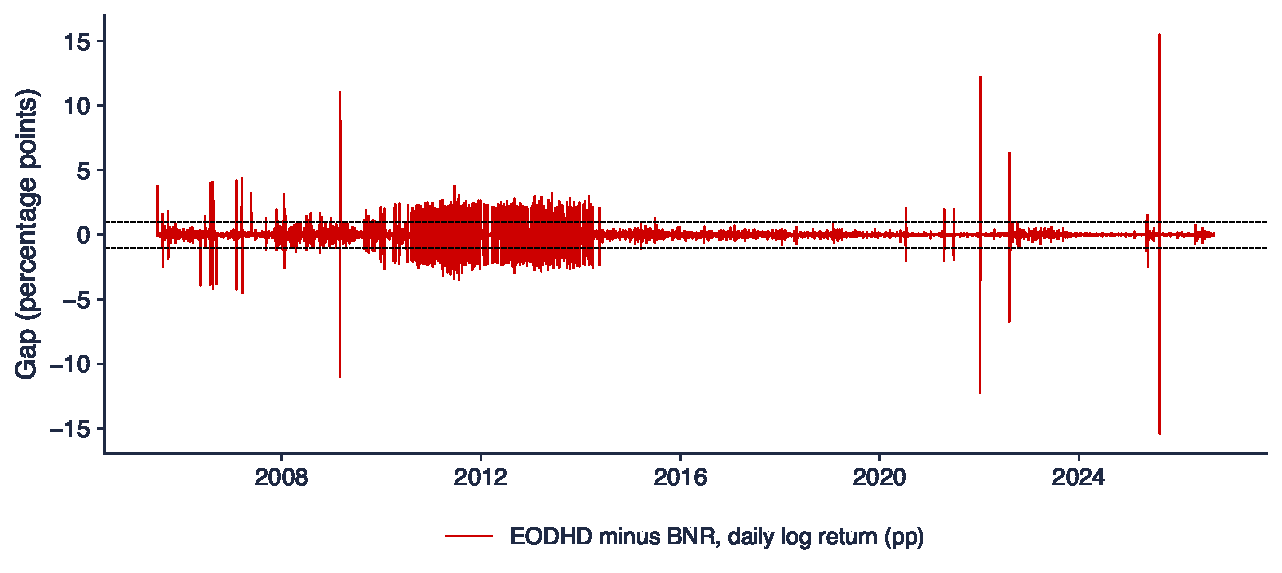
\includegraphics[width=0.96\textwidth,height=0.48\textheight,keepaspectratio]{ch1_sem_b1.pdf}
\end{center}
\vspace{-2mm}
\begin{itemize}
    \item 5\,154 common days; on 412 of them (8.0\%) the gap exceeds one percentage point; most in 2011 (107 days)
    \item Largest gaps: 13 August 2025 (EODHD $15.4\%$, BNR $-0.10\%$), 14 August 2025 (EODHD $-15.4\%$, BNR $-0.01\%$)
    \item Volatility: BNR 4.5\%, EODHD 13.4\%, EODHD without the bad days 4.7\%
    \item Interpretation: the BNR rate, the primary source of the number; the EODHD series would multiply the measured currency risk by 3.0
\end{itemize}\quantlet{SFM\_ch1\_seminar}{\qlurl{SFM_ch1_seminar}}
\end{frame}

\begin{frame}{B2: Is the Mean Return of the BET Positive? [Solved]}
\itemsize{\footnotesize}
\begin{itemize}
\item \textbf{Question}: is the mean daily return of the BET significantly different from zero over 2015--2026?
\item \textbf{Inputs}: BET closes, 2015--2026, daily log returns in \%
\item \textbf{Tasks}
\begin{enumerate}
    \item Compute the mean, standard deviation, skewness, excess kurtosis, minimum (with its date) and maximum of the daily log returns.
    \item Annualise the mean and the standard deviation with the actual number of observations per year.
    \item Compute the standard error of the annual mean, its 95\% CI and the $z$ statistic of $H_0$: mean $= 0$.
    \item Interpretation: does the histogram look like the Normal distribution?
    \item Interpretation: what does the confidence interval tell an investor?
\end{enumerate}
\item \textbf{Report}: a table of statistics, the CI, $z$ and $p$, two sentences of interpretation
\item Notebook: section B2
\end{itemize}
\end{frame}

\begin{frame}{B2: Solution [Solved]}
\itemsize{\footnotesize}
\begin{columns}[T]
\begin{column}{0.50\textwidth}
\begin{center}
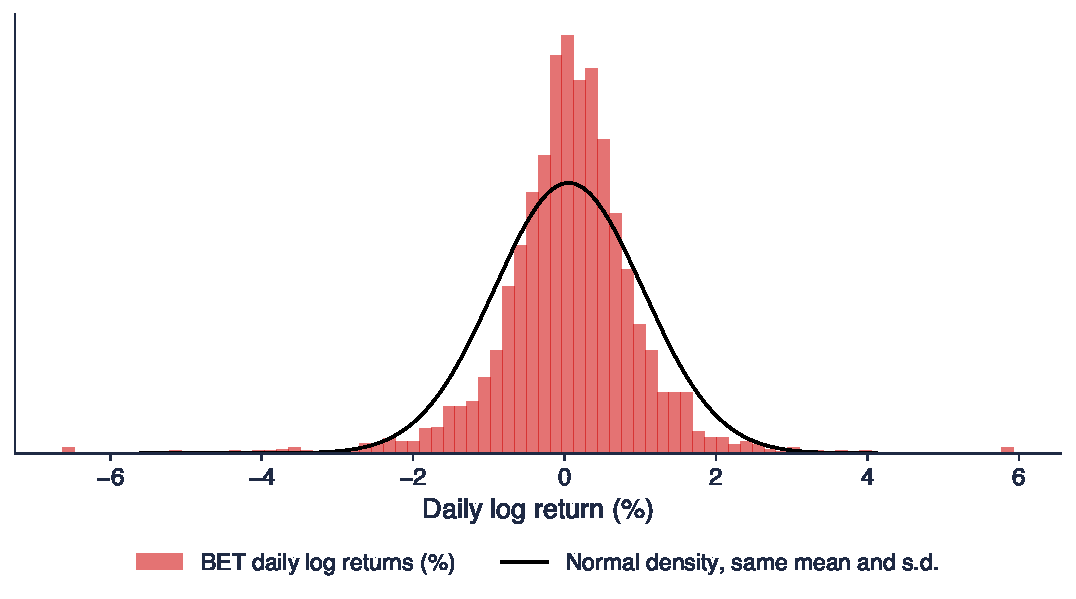
\includegraphics[width=1.0\textwidth,height=0.55\textheight,keepaspectratio]{ch1_sem_b2.pdf}
\end{center}
\vspace{-2mm}

\end{column}
\begin{column}{0.48\textwidth}
\begin{itemize}
    \item $n = 2\,925$ days, 250 a year; mean $0.053\%$, s.d. $0.98\%$
    \item Skewness $-1.41$, excess kurtosis $17.8$; worst day $-11.9\%$ on 19 December 2018, best $6.8\%$
    \item Annual: mean 13.2\%, volatility 15.5\%; SE $= 15.5/\sqrt{11.7} = 4.5\%$
    \item 95\% CI [4.3\%, 22.1\%]; $z = 2.91$, $p = 0.004$: we reject a zero mean at 5\%
    \item Interpretation: a taller centre and heavier tails than the Normal distribution; the mean is positive, but anywhere between 4.3\% and 22.1\% a year
\end{itemize}
\end{column}
\end{columns}\quantlet{SFM\_ch1\_seminar}{\qlurl{SFM_ch1_seminar}}
\end{frame}

\begin{frame}{B3: Four More Markets [Proposed]}
\itemsize{\footnotesize}
\begin{itemize}
\item \textbf{Question}: which of the S\&P 500, DAX, Bitcoin and Banca Transilvania have a mean return significantly above zero?
\item \textbf{Inputs}: daily log returns, 2015--2026, each on its own calendar; model: B2
\item \textbf{Tasks}
\begin{enumerate}
    \item Repeat steps 1--3 of B2 for each of the four series.
    \item Put the annual mean, the volatility, the CI and $p$ of all five series (with the BET) in one table.
    \item Interpretation: why is the interval of Bitcoin so much wider than that of the S\&P 500, although both cover the same years?
\end{enumerate}
\item \textbf{Report}: one table and two sentences
\item Notebook: section B3
\end{itemize}
\end{frame}

\ifsolutions
\begin{frame}{B3: Solution [Proposed]}
\itemsize{\footnotesize}
\begin{center}
\footnotesize
\begin{tabular}{lrrrrr}
\toprule
Series & Mean \% & Vol. \% & SE \% & 95\% CI & $p$ \\
\midrule
BET & $13.2$ & $15.5$ & $4.5$ & [$4.3$, $22.1$] & $0.004$ \\
S\&P 500 & $11.2$ & $17.7$ & $5.2$ & [$1.1$, $21.4$] & $0.030$ \\
DAX & $8.1$ & $19.1$ & $5.6$ & [$-2.8$, $19.1$] & $0.144$ \\
Bitcoin & $47.4$ & $66.7$ & $19.5$ & [$9.2$, $85.6$] & $0.015$ \\
Banca Transilvania & $24.2$ & $25.5$ & $7.5$ & [$9.6$, $38.8$] & $0.001$ \\
\bottomrule
\end{tabular}
\end{center}
\begin{itemize}
    \item Significant at 5\%: every series whose interval excludes zero; the DAX interval contains zero
    \item Interpretation: SE $= \sigma_{\text{year}}/\sqrt{Y}$ with the same $Y$; Bitcoin's volatility is 3.8 times that of the S\&P 500, and so is the width of its interval
\end{itemize}\quantlet{SFM\_ch1\_seminar}{\qlurl{SFM_ch1_seminar}}
\end{frame}
\fi

\begin{frame}{B4: How Precise Is a Sharpe Ratio? [Solved]}
\itemsize{\footnotesize}
\begin{itemize}
\item \textbf{Question}: how precisely is the Sharpe ratio of the S\&P 500 estimated from 2015--2026 data?
\item \textbf{Inputs}: S\&P 500 closes, daily simple returns, $r_f = 0$
\item \textbf{Tasks}
\begin{enumerate}
    \item Compute the daily mean, standard deviation and Sharpe ratio, and annualise the Sharpe ratio.
    \item Compute the standard error of \refLo{} and the 95\% CI.
    \item Bootstrap the Sharpe ratio with 2000 resamples of the days and take the 2.5\% and 97.5\% percentiles.
    \item Interpretation: could the true Sharpe ratio of the S\&P 500 be below 0.25?
\end{enumerate}
\item \textbf{Report}: the Sharpe ratio, two intervals and one sentence
\item Notebook: section B4
\end{itemize}
\end{frame}

\begin{frame}{B4: Solution [Solved]}
\itemsize{\footnotesize}
\begin{columns}[T]
\begin{column}{0.50\textwidth}
\begin{center}
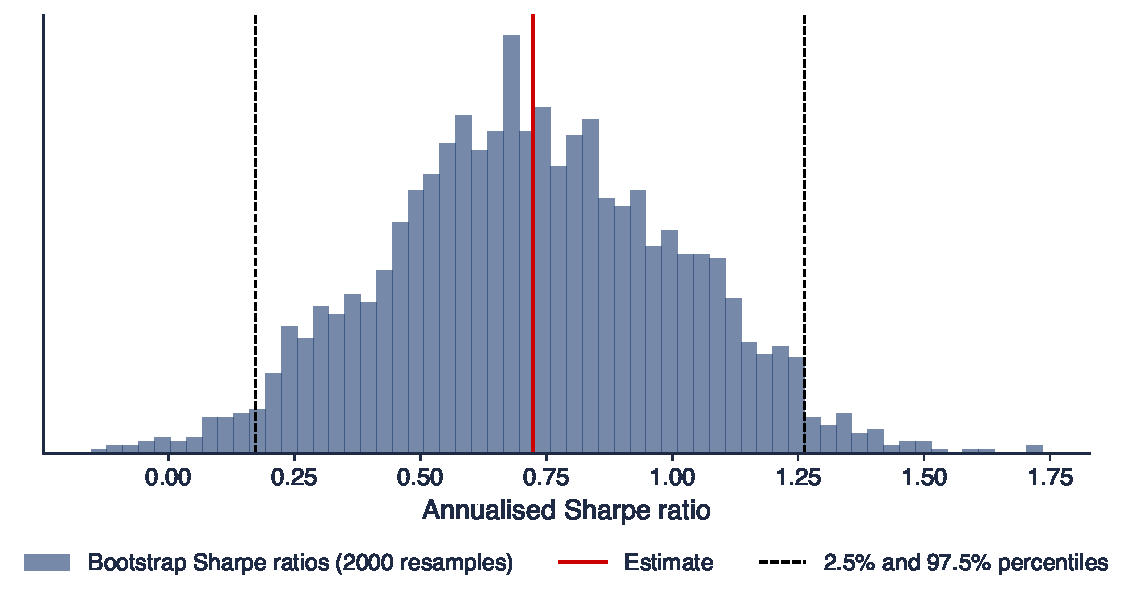
\includegraphics[width=1.0\textwidth,height=0.55\textheight,keepaspectratio]{ch1_sem_b4.pdf}
\end{center}
\vspace{-2mm}

\end{column}
\begin{column}{0.48\textwidth}
\begin{itemize}
    \item $n = 2\,943$, $q = 251.5$; daily mean $0.0508\%$, s.d. $1.113\%$, daily SR $0.0457$
    \item Annual SR $= 0.0457 \times 15.86 = 0.72$
    \item Lo: SE $= \sqrt{(1 + 0.0457^2/2)/2\,943} \times 15.86 = 0.29$; CI [$0.15$, $1.30$]
    \item Bootstrap: [$0.17$, $1.26$], very close
    \item Interpretation: yes; every value from $0.17$ to $1.26$ is compatible with the data
\end{itemize}
\end{column}
\end{columns}\quantlet{SFM\_ch1\_seminar}{\qlurl{SFM_ch1_seminar}}
\end{frame}

\begin{frame}{B5: Is Banca Transilvania Better than the BET? [Proposed]}
\itemsize{\footnotesize}
\begin{itemize}
\item \textbf{Question}: is the Sharpe ratio of TLV significantly higher than that of the BET index?
\item \textbf{Inputs}: BET close and TLV adjusted close, 2015--2026, joined on common days first; model: B4
\item \textbf{Tasks}
\begin{enumerate}
    \item Join the two price series on their common days, then compute daily simple returns.
    \item Compute both annualised Sharpe ratios with their Lo standard errors.
    \item Bootstrap the difference of the two Sharpe ratios, resampling the same days for both series.
    \item Interpretation: why must the days be resampled in pairs?
\end{enumerate}
\item \textbf{Report}: two Sharpe ratios, the difference with its interval, one sentence
\item Notebook: section B5
\end{itemize}
\end{frame}

\ifsolutions
\begin{frame}{B5: Solution [Proposed]}
\itemsize{\footnotesize}
\begin{itemize}
    \item 2\,674 common days; BET SR $0.93$ (SE $0.29$), TLV SR $1.08$ (SE $0.29$)
    \item Difference TLV $-$ BET $= 0.15$; paired bootstrap 95\% interval [$-0.24$, $0.53$], contains zero
    \item No significant difference
    \item Interpretation: the two return series are correlated ($\rho = 0.76$); resampling days in pairs keeps this correlation, which makes the difference more precise than two separate intervals suggest
\end{itemize}\quantlet{SFM\_ch1\_seminar}{\qlurl{SFM_ch1_seminar}}
\end{frame}
\fi

\begin{frame}{B6: The Deepest Fall of the BET [Solved]}
\itemsize{\footnotesize}
\begin{itemize}
\item \textbf{Question}: what were the depth and the duration of the worst fall of the BET since its launch?
\item \textbf{Inputs}: official BET closes since 19 September 1997; for the Calmar ratio, 2015--2026
\item \textbf{Tasks}
\begin{enumerate}
    \item Compute the drawdown series and the maximum drawdown with the dates of the peak, the trough and the recovery.
    \item Compute the gain needed to recover from the trough and the share of days spent more than 20\% below the peak.
    \item Compute the CAGR, the MDD and the Calmar ratio over 2015--2026.
    \item Interpretation: what does the drawdown add to what the volatility already tells us?
\end{enumerate}
\item \textbf{Report}: the MDD with three dates, two percentages, three indicators, one sentence
\item Notebook: section B6
\end{itemize}
\end{frame}

\begin{frame}{B6: Solution [Solved]}
\itemsize{\footnotesize}
\begin{center}
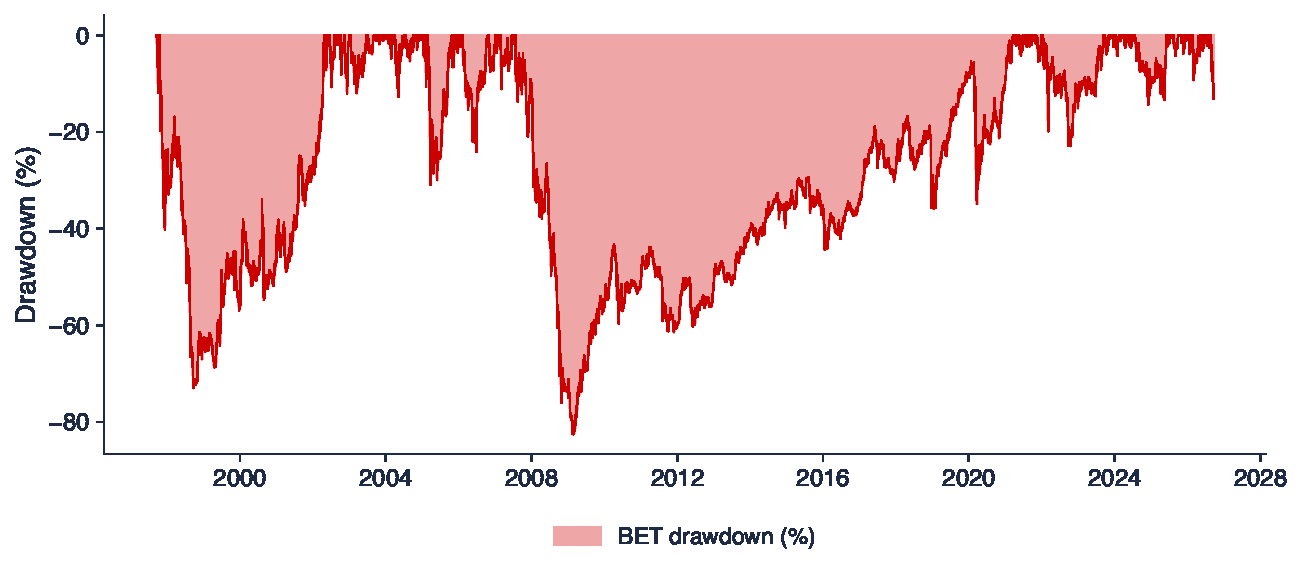
\includegraphics[width=0.96\textwidth,height=0.48\textheight,keepaspectratio]{ch1_sem_b6.pdf}
\end{center}
\vspace{-2mm}
\begin{itemize}
    \item MDD $-82.5\%$: from 10\,814 points on 24 July 2007 to 1\,887 on 25 February 2009; the old peak was regained on 16 March 2021, after 13.6 years
    \item From the trough, a gain of $473\%$ was needed; 56\% of all days were more than 20\% below the peak
    \item 2015--2026: CAGR 14.1\%, MDD $-31.1\%$ (23 January 2020 to 23 March 2020), Calmar $= 14.1/31.1 = 0.45$
    \item Interpretation: volatility ignores the order of returns; the drawdown shows how long an investor stays under water
\end{itemize}\quantlet{SFM\_ch1\_seminar}{\qlurl{SFM_ch1_seminar}}
\end{frame}

\begin{frame}{B7: Bitcoin, OMV Petrom and the Volatility Drag [Proposed]}
\itemsize{\footnotesize}
\begin{itemize}
\item \textbf{Question}: what do the drawdowns and the volatility drag show for Bitcoin and SNP?
\item \textbf{Inputs}: Bitcoin close and SNP adjusted close, 2015--2026; model: B6
\item \textbf{Tasks}
\begin{enumerate}
    \item Compute the MDD of each series with the dates of the peak, the trough and the recovery.
    \item Compute the CAGR and the Calmar ratio of each series.
    \item Compute the arithmetic annual mean of simple returns, the annual mean of log returns and their difference.
    \item Compare the difference with $\sigma^2/2$, using the annual volatility of simple returns.
    \item Interpretation: for which asset does the drag matter for a long-term investor?
\end{enumerate}
\item \textbf{Report}: a table with MDD, dates, CAGR, Calmar, the two means, the drag and $\sigma^2/2$, one sentence
\item Notebook: section B7
\end{itemize}
\end{frame}

\ifsolutions
\begin{frame}{B7: Solution [Proposed]}
\itemsize{\footnotesize}
\begin{center}
\footnotesize
\begin{tabular}{lrrrrrrr}
\toprule
Series & MDD \% & CAGR \% & Calmar & Arith. \% & Log \% & Drag \% & $\sigma^2/2$ \% \\
\midrule
Bitcoin & $-83.4$ & $60.6$ & $0.73$ & $69.5$ & $47.4$ & $22.13$ & $21.93$ \\
OMV Petrom & $-45.4$ & $19.7$ & $0.43$ & $20.8$ & $18.0$ & $2.73$ & $2.71$ \\
\bottomrule
\end{tabular}
\end{center}
\begin{itemize}
    \item Bitcoin: 16 December 2017 to 15 December 2018, recovered on 30 November 2020; SNP: 1 January 2015 to 12 February 2016, recovered on 20 September 2018
    \item The drag and $\sigma^2/2$ differ by at most 0.20 percentage points
    \item Interpretation: for Bitcoin the drag removes 32\% of the arithmetic mean; for SNP it is small
\end{itemize}\quantlet{SFM\_ch1\_seminar}{\qlurl{SFM_ch1_seminar}}
\end{frame}
\fi


%=============================================================================
\section{Part C: Open Questions and AI Critique}
%=============================================================================

\begin{frame}{C1: Do Sharpe Ratios Persist? [Proposed]}
\itemsize{\footnotesize}
\begin{itemize}
\item \textbf{Question}: does a BVB stock with a high Sharpe ratio in 2015--2020 also have a high one in 2021--2026?
\item \textbf{Inputs}: adjusted closes of TLV, SNP, BRD, TGN, SNG, SNN, 2015--2026; models: B4, B6
\item \textbf{Tasks}
\begin{enumerate}
    \item Compute the annualised Sharpe ratio and its standard error for each stock in each half.
    \item Compute the Spearman rank correlation between the Sharpe ratios of the two halves.
    \item Propose one way to make the answer more reliable (more stocks, other indicators, other windows).
    \item Interpretation: what can six stocks tell us about persistence?
\end{enumerate}
\item \textbf{Report}: a table, the rank correlation with its $p$-value, a short plan for a project
\item Notebook: section C1
\end{itemize}
\end{frame}

\ifsolutions
\begin{frame}{C1: Reference Analysis [Proposed]}
\itemsize{\footnotesize}
\begin{center}
\footnotesize
\begin{tabular}{lrrrr}
\toprule
Stock & SR 2015--2020 & SE & SR 2021--2026 & SE \\
\midrule
Banca Transilvania & $0.91$ & $0.41$ & $1.34$ & $0.42$ \\
OMV Petrom & $0.26$ & $0.41$ & $1.75$ & $0.42$ \\
BRD & $0.71$ & $0.41$ & $0.96$ & $0.42$ \\
Transgaz & $0.63$ & $0.41$ & $1.27$ & $0.42$ \\
Romgaz & $0.52$ & $0.41$ & $1.63$ & $0.42$ \\
Nuclearelectrica & $1.31$ & $0.41$ & $1.23$ & $0.42$ \\
\bottomrule
\end{tabular}
\end{center}
\begin{itemize}
    \item Spearman rank correlation $-0.71$ ($p = 0.11$, $n = 6$): no evidence of persistence; if anything, a reversal
    \item Each half-sample Sharpe ratio has a standard error of about $0.41$: rankings are mostly noise
    \item Project directions: all liquid BVB stocks, rolling three-year windows, Sortino and Calmar, comparison with \refHLZ
\end{itemize}\quantlet{SFM\_ch1\_seminar}{\qlurl{SFM_ch1_seminar}}
\end{frame}
\fi

\begin{frame}{C2: Audit an AI Answer [Proposed]}
\itemsize{\scriptsize}
\begin{itemize}
    \item A student asked an AI assistant: ``Compare the risk and the performance of Bitcoin and the BET in 2015--2026.'' The answer:
    \item \aiprompt{(a) Bitcoin's daily volatility is 3.49\%, so its annual volatility is 3.49\% x sqrt(252) = 55.4\%.}
    \item \aiprompt{(b) Bitcoin's Sharpe ratio (1.05) is higher than the BET's (0.93), which proves that Bitcoin is the better investment.}
    \item \aiprompt{(c) Bitcoin's maximum drawdown is its worst daily return, -46.5\%.}
    \item \aiprompt{(d) For a 50/50 portfolio, the log return is exactly the average of the two log returns.}
    \item \aiprompt{(e) For BVB stocks such as TLV I used the close column, which is the official price.}
    \item Tasks
    \begin{itemize}
        \item 1. For each statement, say whether it is correct; if not, give the correct statement and, where possible, the correct number from the notebook (section C2).
        \item 2. Report: a list of five verdicts with one line of justification each.
    \end{itemize}
\end{itemize}
\end{frame}

\ifsolutions
\begin{frame}{C2: Solution [Proposed]}
\itemsize{\footnotesize}
\begin{itemize}
    \item (a) Wrong factor: Bitcoin trades about 365 days a year; $3.49\% \times \sqrt{365} = 66.7\%$, not 55.4\%
    \item (b) Not proved: SE $\approx 0.29$ for each Sharpe ratio, so the gap of the two estimates is well within the noise; and past Sharpe ratios do not guarantee future ones
    \item (c) Wrong definition: MDD is the worst peak-to-trough fall, $-83.4\%$; the worst day was $-46.5\%$ (log return)
    \item (d) Wrong: $R_p = \sum_i w_i R_i$ is exact; $r_p = \ln(\sum_i w_i e^{r_i})$ differs from $\sum_i w_i r_i$
    \item (e) Wrong column: TLV's close jumps by $+230\%$ (log) on 16 August 2022, a share consolidation; volatility from the close 73.1\% vs 25.5\% from the adjusted close
\end{itemize}\quantlet{SFM\_ch1\_seminar}{\qlurl{SFM_ch1_seminar}}
\end{frame}
\fi


%=============================================================================
\section{Wrap-Up}
%=============================================================================

\begin{frame}{What You Should Take from Today}
\itemsize{\small}
\begin{itemize}
    \item Check the data before computing: source, adjusted prices, a second series
    \item Log returns add over time; simple returns add across assets
    \item Mean returns and Sharpe ratios come with wide intervals: report them
    \item The drawdown and the volatility drag show what the volatility alone hides
    \item An AI answer is a draft: check every factor, definition and column
\end{itemize}
\end{frame}

\begin{frame}{After the Seminar}
\itemsize{\small}
\begin{itemize}
    \item Lecture 1 develops each topic of today: data quality, returns, annualisation, descriptive statistics and performance indicators
    \item Try the [Proposed] tasks in the notebook; the solutions are discussed in class
    \item C1 can grow into a team project: more stocks, rolling windows, other indicators
    \item Reading: \refFHH, Ch.~11; exercises with solutions: \refFHHex
\end{itemize}
\end{frame}


%=============================================================================
\section{References}
%=============================================================================

\begin{frame}{References}
\itemsize{\tiny}
\begin{itemize}
    \item Borak, S., Härdle, W.K., López-Cabrera, B. (2013). \href{https://doi.org/10.1007/978-3-642-33929-5}{\textit{Statistics of Financial Markets: Exercises and Solutions}}, 2nd ed. Springer.
    \item Franke, J., Härdle, W.K., Hafner, C.M. (2019). \href{https://doi.org/10.1007/978-3-030-13751-9}{\textit{Statistics of Financial Markets: An Introduction}}, 5th ed. Springer.
    \item Harvey, C.R., Liu, Y., Zhu, H. (2016). \href{https://doi.org/10.1093/rfs/hhv059}{\ldots and the cross-section of expected returns}. \textit{Review of Financial Studies}, 29(1), 5--68.
    \item Lo, A.W. (2002). \href{https://doi.org/10.2469/faj.v58.n4.2453}{The statistics of Sharpe ratios}. \textit{Financial Analysts Journal}, 58(4), 36--52.
    \item Sharpe, W.F. (1994). \href{https://doi.org/10.3905/jpm.1994.409501}{The Sharpe ratio}. \textit{Journal of Portfolio Management}, 21(1), 49--58.
    \item Sortino, F.A., van der Meer, R. (1991). \href{https://doi.org/10.3905/jpm.1991.409343}{Downside risk}. \textit{Journal of Portfolio Management}, 17(4), 27--31.
\end{itemize}
\end{frame}

\end{document}
